\section{Triển khai ứng dụng}
\label{sec:trien_khai}

\subsection{Kiến trúc ứng dụng}

Nhóm xây dựng ứng dụng web bằng Streamlit để minh họa cách ba mô hình được đánh giá ở Chương~\ref{sec:thuc_nghiem} phân loại từng ảnh. Hai mô hình SVM, gồm SVM RBF kết hợp PCA và SVM tuyến tính, được huấn luyện trên nhánh \emph{direct}. Mô hình hồi quy logistic cơ sở được huấn luyện trên nhánh \emph{padding}. Mỗi mô hình được lưu thành một quy trình xử lý gồm bộ chuẩn hóa và bộ phân loại. Quy trình của SVM RBF còn chứa phép chiếu PCA xuống 256 chiều.

Sau khi người dùng tải ảnh lên, ứng dụng xử lý ảnh theo các bước sau.

\begin{enumerate}
  \item Giải mã ảnh bằng OpenCV. Nếu tệp không phải ảnh hợp lệ, ứng dụng báo lỗi và dừng xử lý.
  \item Chuẩn hóa kích thước ảnh về 224 $\times$ 224 điểm ảnh theo nhánh mà mô hình đã dùng khi huấn luyện. Với hai mô hình SVM, ứng dụng co giãn trực tiếp. Với hồi quy logistic, ứng dụng giữ tỷ lệ khung ảnh rồi đệm viền xám như ở Đoạn mã~\ref{lst:padding}. Cả hai nhánh dùng cùng quy tắc nội suy với bước tiền xử lý dữ liệu huấn luyện: nội suy song khối khi cả hai chiều nhỏ hơn 224 điểm ảnh, nội suy theo diện tích trong các trường hợp còn lại.
  \item Chuyển ảnh sang ảnh xám rồi trích xuất HOG với cấu hình ở Chương~\ref{sec:du_lieu}. Ứng dụng kiểm tra vectơ đặc trưng có đúng 26.244 chiều trước khi dự đoán.
  \item Dự đoán bằng cả ba mô hình. Giao diện hiển thị kết quả của mô hình mà người dùng chọn, còn kết quả của hai mô hình còn lại được lưu cho phần đánh giá trong phiên.
  \item Hiển thị nhãn dự đoán và điểm số của sáu lớp dưới dạng biểu đồ cột và bảng. Với hồi quy logistic, điểm số là xác suất do mô hình ước lượng. Với SVM, điểm số là kết quả của hàm softmax áp dụng lên điểm quyết định. Nhãn thuộc nhóm vũ khí được tô màu đỏ, nhãn thuộc nhóm đồ vật thông thường được tô màu xanh.
\end{enumerate}

\begin{lstlisting}[caption={Trích xuất đặc trưng và dự đoán trong ứng dụng web (rút gọn)},label={lst:app}]
def extract_features(img_bgr, branch="direct"):
    height, width = img_bgr.shape[:2]
    interpolation = (cv2.INTER_CUBIC if width < 224 and height < 224
                     else cv2.INTER_AREA)
    if branch == "padding":
        resized = resize_padding(img_bgr, interpolation)
    else:
        resized = cv2.resize(img_bgr, (224, 224), interpolation=interpolation)
    gray = cv2.cvtColor(resized, cv2.COLOR_BGR2GRAY)
    return hog(gray, **HOG_CONFIG).astype(np.float32).reshape(1, -1)

def predict(img_bgr, pipeline, branch="direct"):
    features = extract_features(img_bgr, branch)
    prediction = pipeline.predict(features)[0]
    if hasattr(pipeline, "predict_proba"):     # logistic regression
        return prediction, pipeline.predict_proba(features)[0]
    scores = pipeline.decision_function(features)[0]
    return prediction, softmax(scores)         # SVM: relative scores
\end{lstlisting}

\subsection{Nạp mô hình và lưu vào bộ nhớ đệm}

Ứng dụng dùng bộ nhớ đệm tài nguyên của Streamlit để nạp mỗi mô hình một lần cho mỗi tiến trình. Khi người dùng tải ảnh khác hoặc chuyển giữa các thẻ, ứng dụng dùng lại mô hình đã nạp và chỉ thực hiện tiền xử lý, trích xuất HOG và dự đoán trên ảnh mới.

\subsection{Các chức năng của ứng dụng}

Giao diện có ba thẻ.

\begin{itemize}
  \item \textbf{Thử nghiệm dự đoán.} Người dùng chọn mô hình, tải ảnh lên và xem nhãn dự đoán cùng điểm số của sáu lớp. Sau đó người dùng chọn nhãn đúng của ảnh. Ứng dụng lưu ảnh, nhãn đúng và dự đoán của cả ba mô hình vào trạng thái của phiên làm việc.
  \item \textbf{Báo cáo đánh giá.} Người dùng chọn một trong ba mô hình. Với mô hình được chọn, ứng dụng tính độ chính xác, macro-F1, precision, recall và F1 của từng lớp, cùng ma trận nhầm lẫn trên các ảnh đã ghi nhãn trong phiên. Khi phiên có ít nhất bốn ảnh thuộc ít nhất hai lớp, ứng dụng còn vẽ một đường cong độ chính xác theo $C$. Đường cong này được tính bằng kiểm định chéo bỏ một mẫu (leave-one-out): ứng dụng huấn luyện các mô hình SVM tuyến tính mới trên chính các ảnh của phiên với $C \in \{0{,}01;\ 0{,}1;\ 1;\ 10;\ 100\}$.
  \item \textbf{Phân tích lỗi.} Ứng dụng liệt kê các ảnh trong phiên mà SVM tuyến tính phân loại sai, kèm nhãn đúng và nhãn dự đoán, và thống kê các cặp lớp bị nhầm lẫn.
\end{itemize}

\begin{figure}[H]
    \centering
    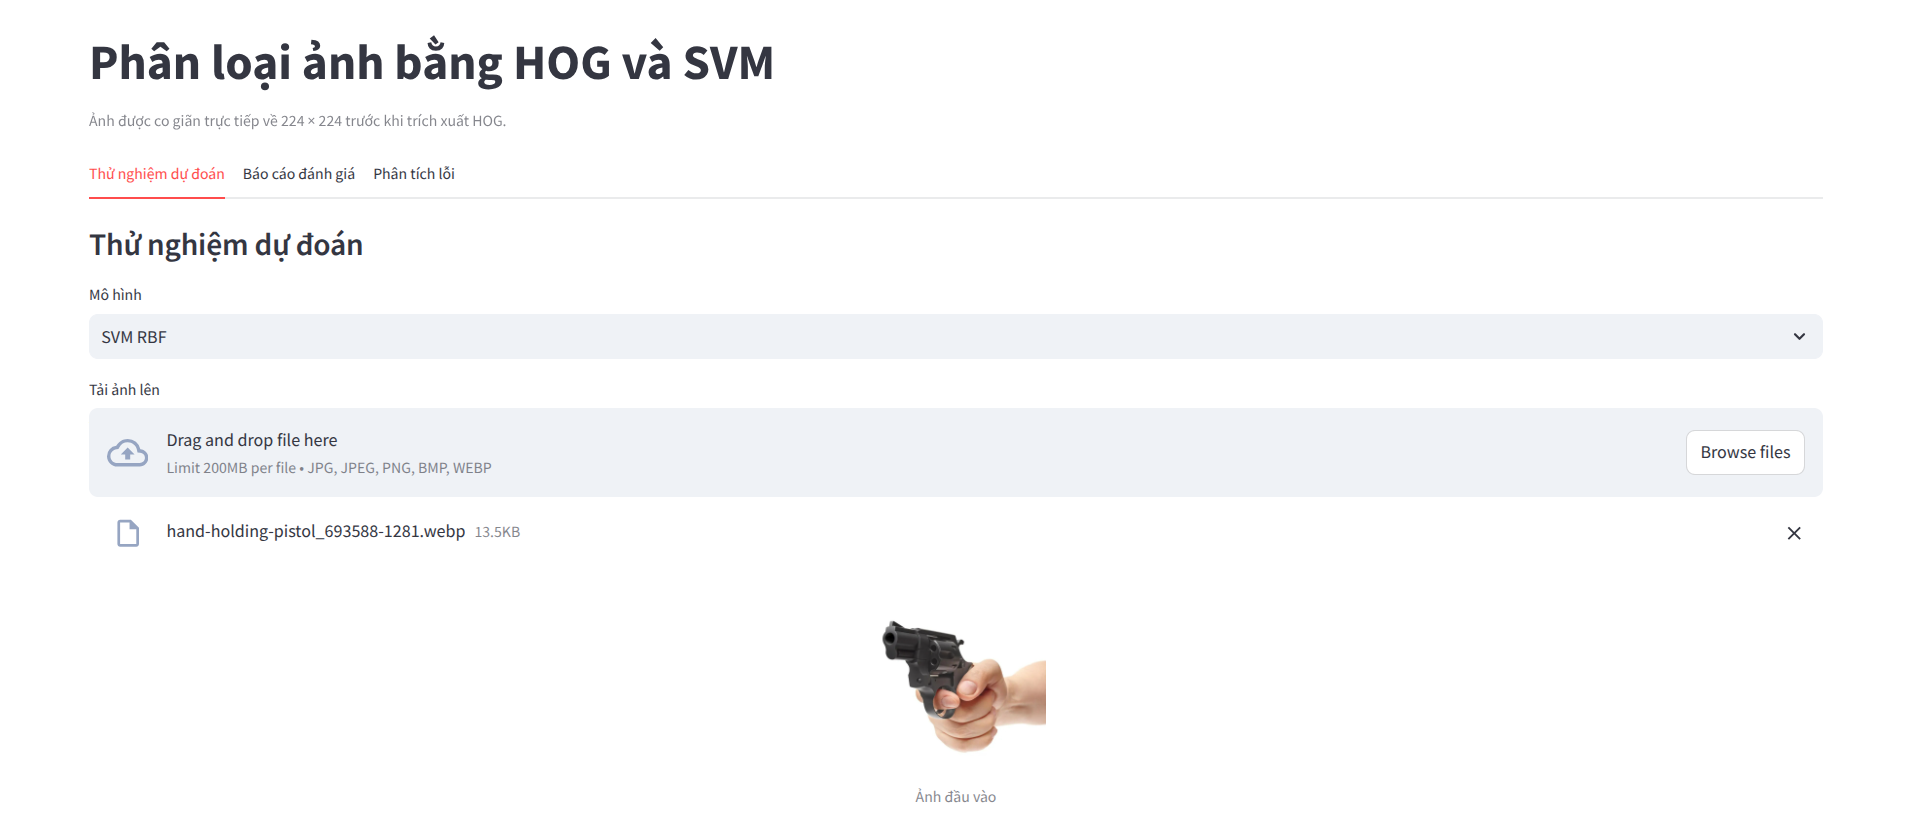
\includegraphics[width=1\linewidth]{image.png}
    \caption{Giao diện ứng dụng web phân loại vật thể}
\end{figure}
\begin{figure}[H]
    \centering
    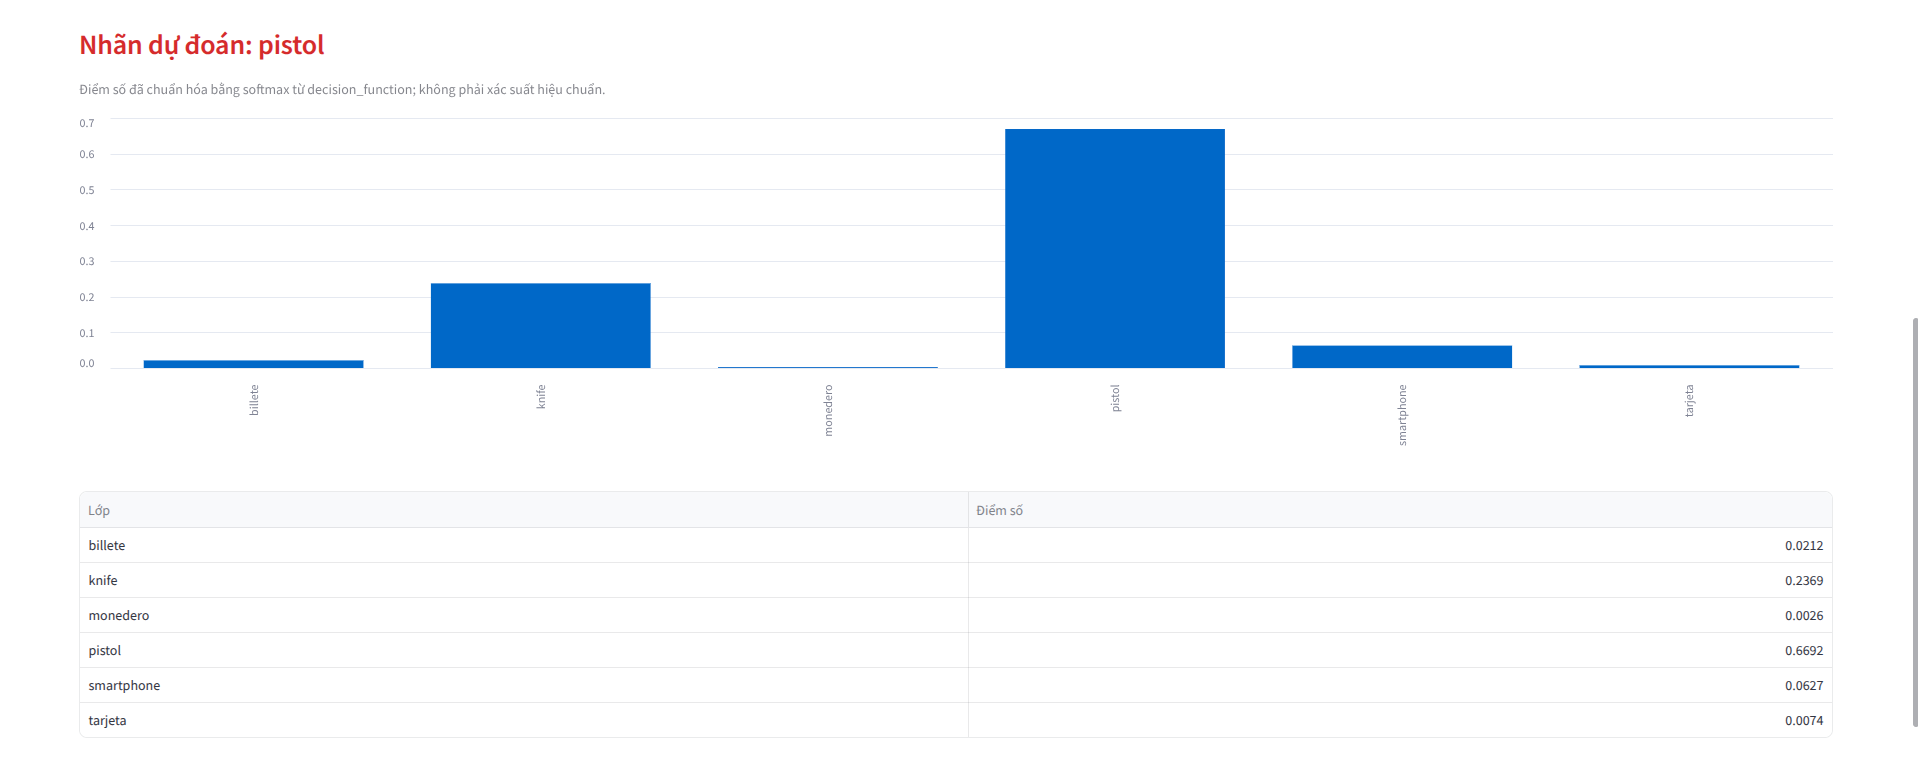
\includegraphics[width=1\linewidth]{image1.png}
    \caption{Giao diện kết quả dự đoán của mô hình}
\end{figure}

\subsection{Đóng gói bằng Docker}

Nhóm đóng gói ứng dụng bằng Docker trên môi trường Python 3.12. Ảnh Docker chỉ chứa mã nguồn của ứng dụng, ba mô hình đã huấn luyện và sáu thư viện cần cho việc dự đoán. Phiên bản của các thư viện được cố định. Riêng scikit-learn được giữ ở phiên bản 1.6.1, là phiên bản đã dùng để lưu mô hình, nhằm tránh lỗi khi nạp mô hình bằng phiên bản khác. Ứng dụng chạy bằng tài khoản không có quyền quản trị, và Docker định kỳ kiểm tra ứng dụng còn phản hồi hay không. Người dùng có thể xây dựng và chạy ứng dụng bằng hai lệnh dưới đây, sau đó mở trình duyệt tại cổng 8501.

\begin{lstlisting}[language=bash,numbers=none,caption={Xây dựng và chạy ứng dụng bằng Docker}]
docker build -t sohas-weapon-classification .
docker run --rm -p 8501:8501 sohas-weapon-classification
\end{lstlisting}

\subsection{Đánh giá khả năng sử dụng thực tế}

Ứng dụng minh họa quá trình phân loại trên từng ảnh. Khi đọc kết quả trên giao diện, cần lưu ý bốn giới hạn.

\begin{itemize}
  \item \textbf{Phạm vi đầu vào.} Kết quả thực nghiệm dựa trên ảnh đã cắt quanh vật thể. Với toàn bộ khung hình camera, cần xác định vùng chứa vật thể trước khi đưa vào bộ phân loại.
  \item \textbf{Điểm số trên giao diện.} Với hai mô hình SVM, ứng dụng áp dụng softmax lên điểm quyết định để hiển thị sáu giá trị có tổng bằng 1. Đây là điểm số tương đối và chưa được hiệu chỉnh, nên không thể đọc như xác suất. Nếu cần xác suất, có thể khảo sát các phương pháp hiệu chỉnh xác suất như Platt scaling. Với hồi quy logistic, giá trị hiển thị là xác suất do mô hình ước lượng. Tuy nhiên, Chương~\ref{sec:thuc_nghiem} cho thấy 51\% ảnh bị phân loại sai trên tập test vẫn được gán xác suất trên 0,9, nên xác suất cao trên giao diện không bảo đảm dự đoán đúng.
  \item \textbf{Đánh giá trong phiên.} Các chỉ số ở thẻ đánh giá và phân tích lỗi được tính trên số ít ảnh mà người dùng tải lên và tự gán nhãn. Vì vậy chúng không thay thế được kết quả trên tập test ở Chương~\ref{sec:thuc_nghiem}. Dữ liệu này cũng mất khi người dùng tải lại trang.
  \item \textbf{Đường cong theo $C$ trong phiên.} Đường cong này mô tả các mô hình mới huấn luyện trên ảnh của phiên. Nó không thay đổi mô hình đang dùng để dự đoán và không thay thế quá trình chọn $C$ trên tập validation ở Chương~\ref{sec:thuc_nghiem}.
\end{itemize}
